\chapter{System Design and Architecture}
\label{chap:design}

\section{System Architecture Overview}
Project FORGE is engineered around a modular, multi-tier decoupled architecture designed to execute on client hardware with zero external runtime dependencies. As illustrated in Figure~\ref{fig:sys_arch}, the system is organized into four distinct conceptual layers:
\begin{enumerate}
    \item \textbf{Presentation \& Input Layer:} Manages player keyboard/mouse inputs, camera positioning, trauma screen shake, floating combat text, and the real-time supervisor Defense Telemetry Overlay.
    \item \textbf{Core Gameplay Engine Layer (Godot 4.x):} Implements 2D kinematic physics, player state transitions (idle, run, attack, dash), adversary finite state machines, hazard hitboxes, and projectile life-cycles.
    \item \textbf{Generative AI \& Adaptation Layer:} Houses the two-stage dungeon layout generator, the pure-GDScript neural network forward pass (\texttt{PPOPolicy}), and the parameter translation logic (\texttt{DifficultyManager}).
    \item \textbf{Telemetry \& Data Persistence Layer:} Continuously collects fine-grained gameplay metrics, executes cold-start aggregation ($CR_0$), and handles client-side JSON serialization.
\end{enumerate}

\begin{figure}[!htbp]
\centering
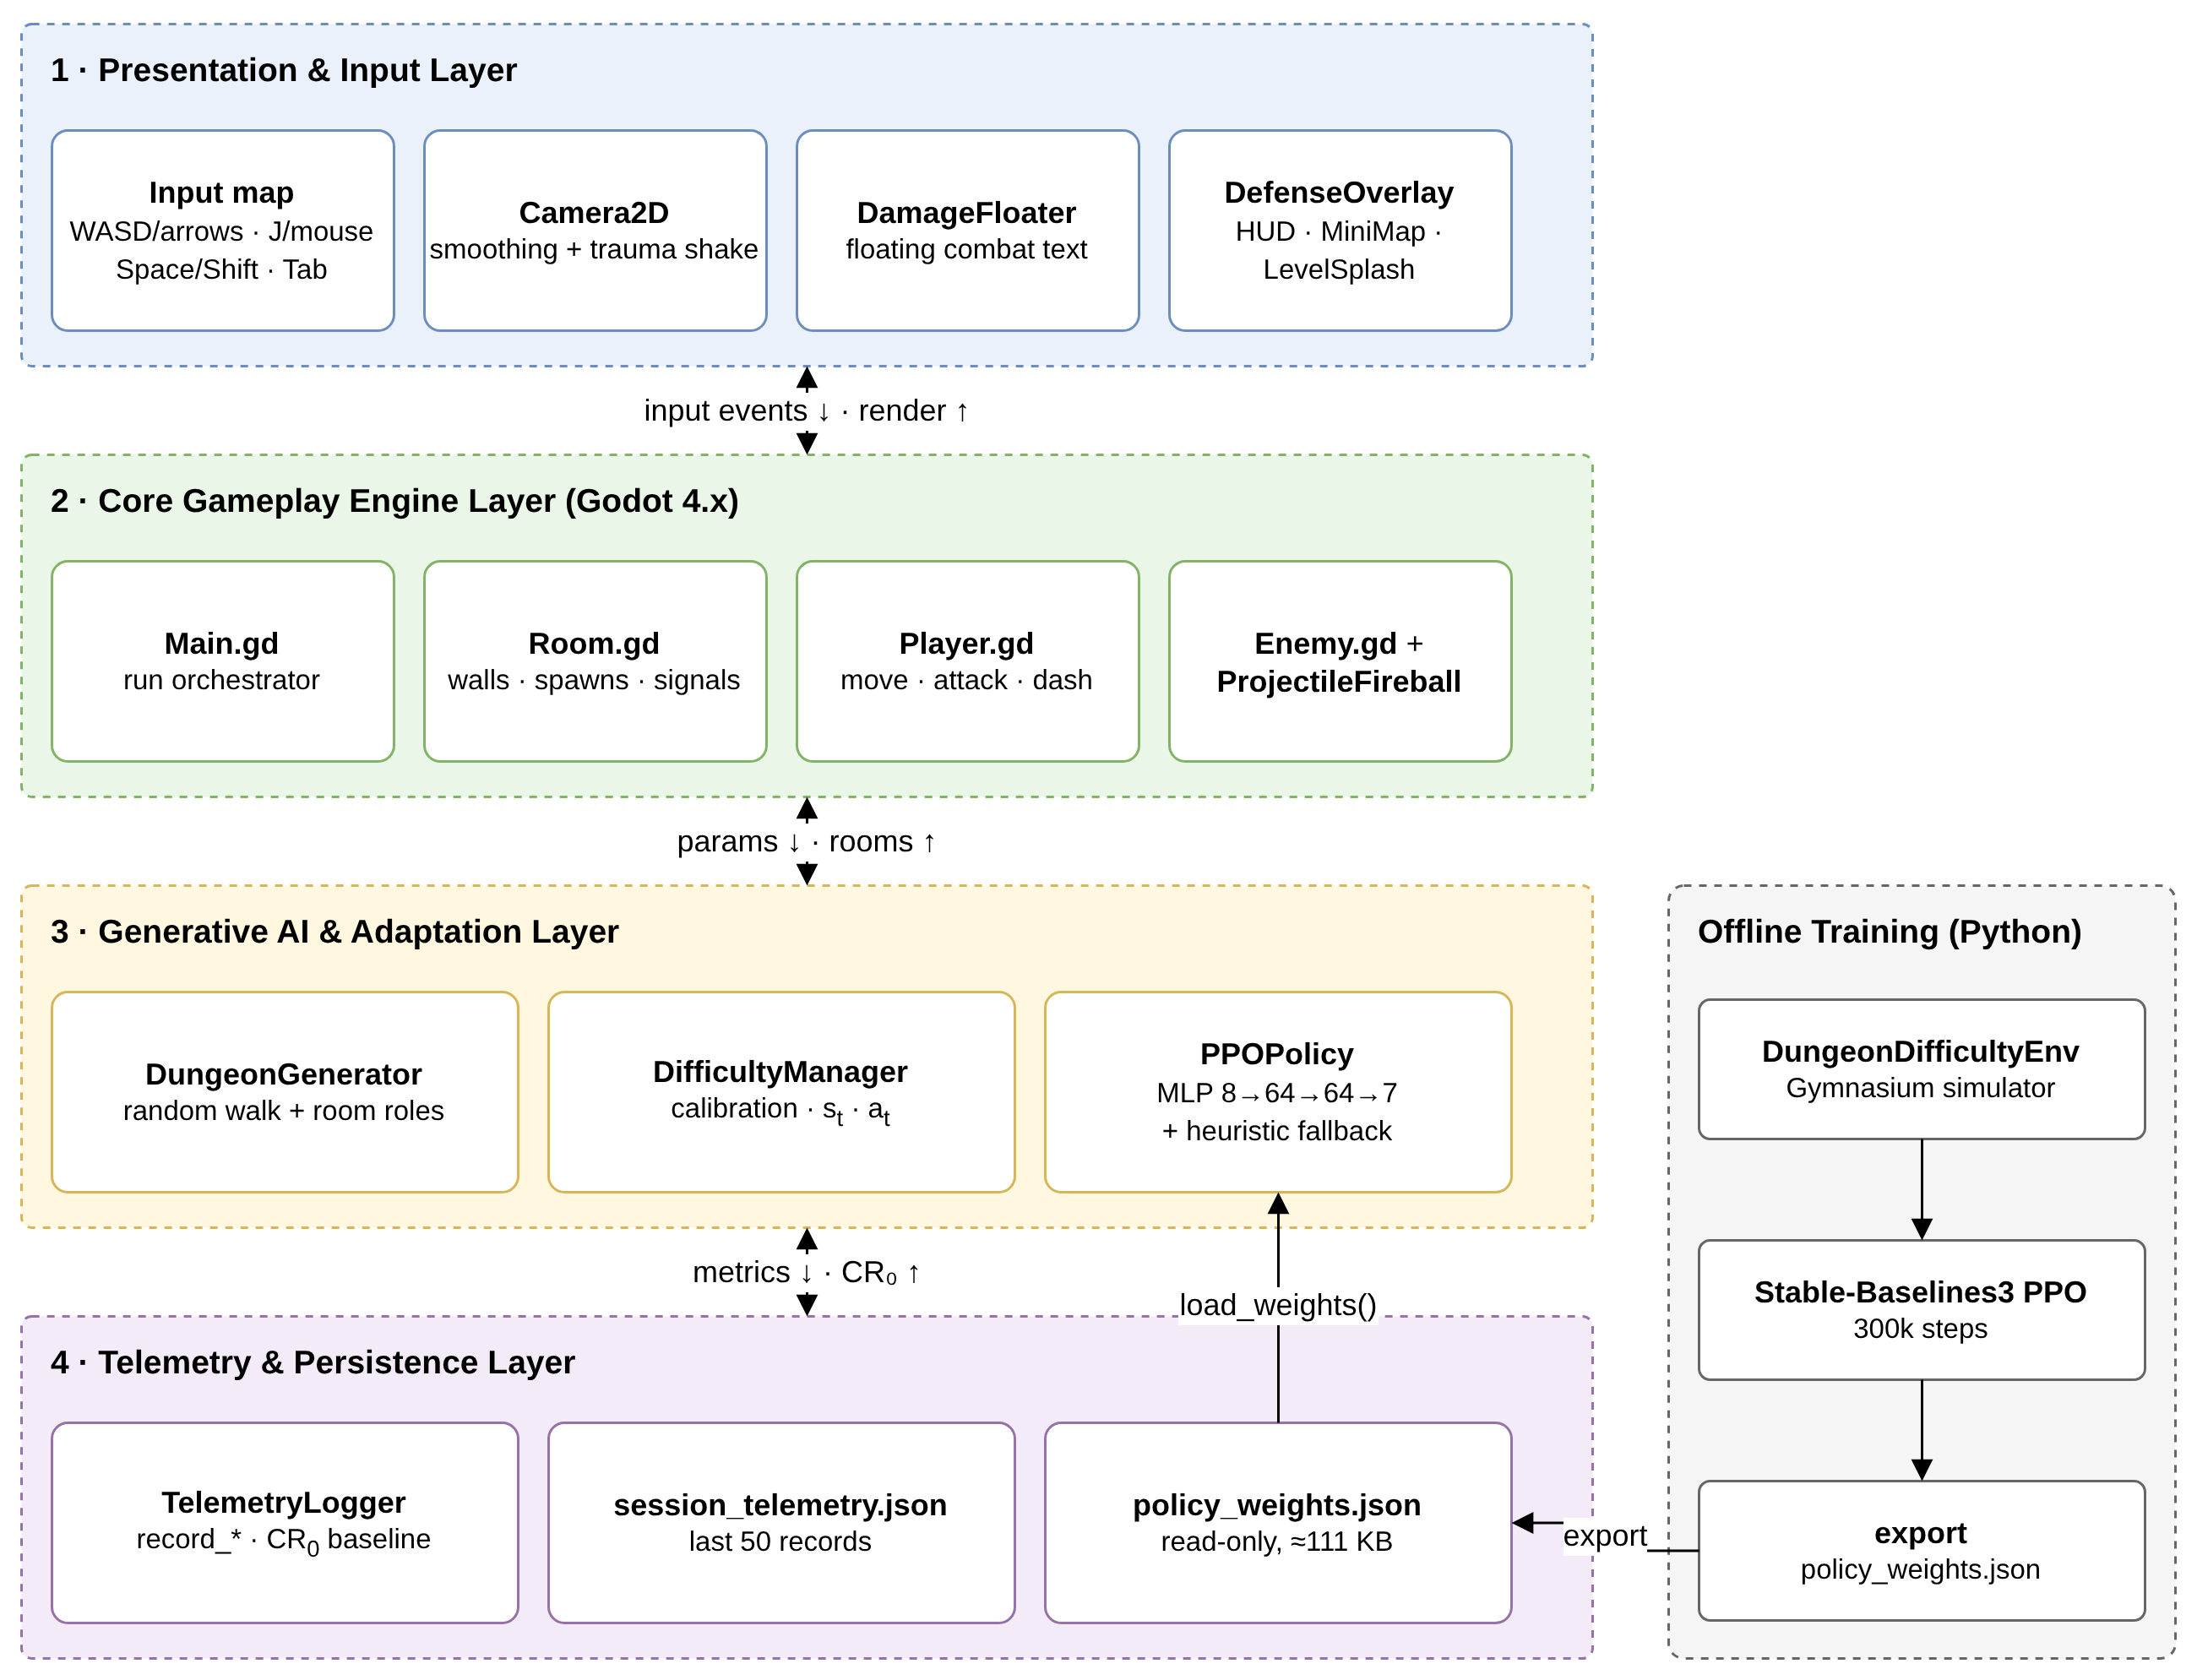
\includegraphics[width=0.95\textwidth]{ThesisFigs/fig_5_1_system_architecture.png}
\caption{Four-Tier System Architecture of Project FORGE}
\label{fig:sys_arch}
\end{figure}

\section{Architectural Components}
The primary responsibilities of the core engine components are detailed below:
\begin{itemize}
    \item \textbf{\texttt{Main.gd}:} The central gameplay orchestrator. Coordinates room transitions, scene loading, camera attachment, player death and respawn cycles, trauma camera shake dampening, and inter-floor progression.
    \item \textbf{\texttt{DifficultyManager.gd}:} Acts as the bridge between raw game parameters and the AI policy. Manages the 5-floor cold-start calibration, scales parameters deterministically under Static Baseline mode, normalizes telemetry observations ($s_t$), and denormalizes PPO actions ($a_t$) into concrete bounds.
    \item \textbf{\texttt{DungeonGenerator.gd}:} Executes Stage 1 generation. Generates a grid of rooms by random walk with branching, opens matching doors between neighbouring rooms, designates the Manhattan-farthest room as the Exit, and assigns the remaining rooms Hazard, Treasure or Combat roles. Because every room is attached to an already placed room, the layout is a connected tree by construction.
    \item \textbf{\texttt{PPOPolicy.gd}:} Contains the neural network forward pass. Loads exported JSON weights, executes the matrix multiplications with $\tanh$ hidden activations in native GDScript, clips the linear output layer to $[-1,1]$ exactly as Stable-Baselines3 does for a deterministic action, and triggers a deterministic heuristic fallback if weights are missing or unparsable.
    \item \textbf{\texttt{TelemetryLogger.gd}:} Operates as an event-driven telemetry sink fed by \texttt{Main.gd}. Accumulates damage dealt, damage taken, deaths, kills, pickups and hazard hits, and at the end of Floor 5 computes $CR_0$ and the training-scale calibration averages that seed $s_0$.
    \item \textbf{\texttt{Enemy.gd} \& \texttt{ProjectileFireball.gd}:} Implements adversary behaviors. Differentiates between Melee Crawlers (chase and bite) and Ranged Pyromancers (kiting and casting telegraphed fireballs).
\end{itemize}

Figure~\ref{fig:low_level_arch} illustrates the low-level component interaction and runtime dataflow architecture, capturing the boundary between offline policy synthesis, automated continuous integration verification, and the real-time Godot 4.x subsystems.

\begin{figure}[!htbp]
\centering
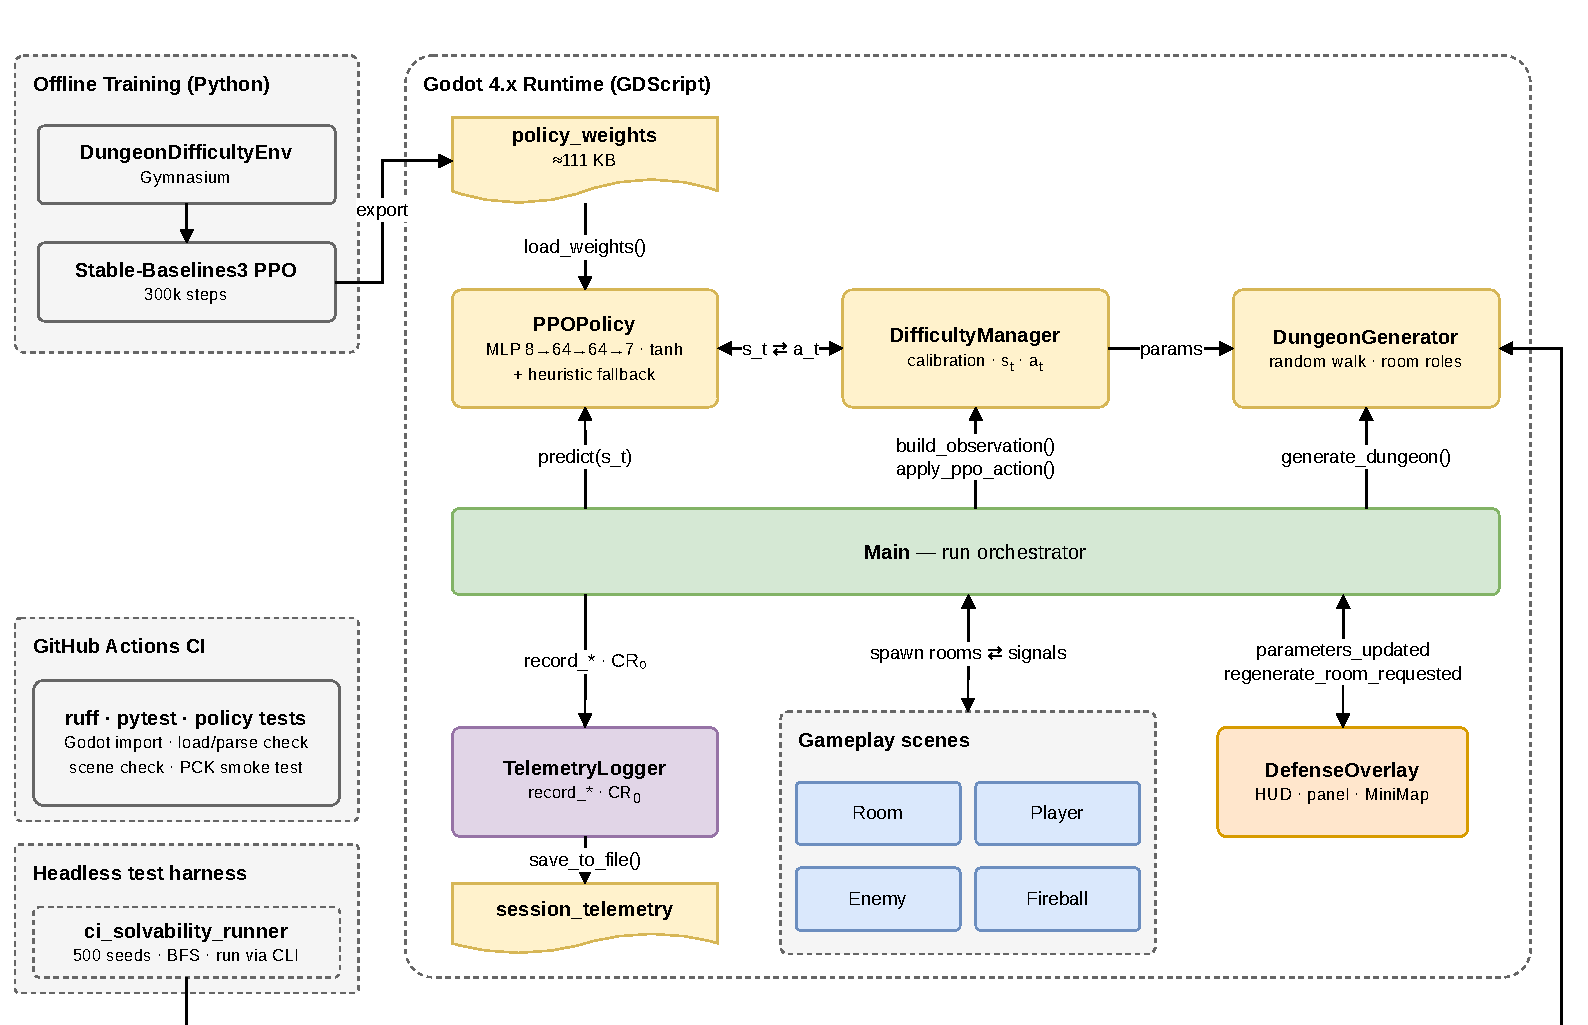
\includegraphics[width=0.95\textwidth]{ThesisFigs/fig_low_level_architecture}
\caption{Low-Level Component Interaction and Runtime Dataflow Architecture}
\label{fig:low_level_arch}
\end{figure}

\section{Interfaces and Data Contracts}

\subsection{Observation Vector Contract ($s_t \in \mathbb{R}^8$)}\label{sec:obs_contract}
At the conclusion of each floor, \texttt{DifficultyManager.gd} packages the player's recent performance into an 8-dimensional normalized observation vector $s_t$:
\begin{equation}
s_t = [s_{\text{time}}, \, s_{\text{deaths}}, \, s_{\text{dmg\_ratio}}, \, s_{\text{hp}}, \, s_{\text{dmg}}, \, s_{\text{haz}}, \, s_{\text{rooms}}, \, s_{\text{level}}]
\label{eq:obs_vector}
\end{equation}
where:
\begin{itemize}
    \item $s_{\text{time}} = \text{clamp}(t_{\text{clear}} / 90.0, 0, 1)$: Normalized floor clearing time, where $t_{\text{clear}}$ is the wall-clock time from floor start to exit ($45$\,s, i.e.\ $7.5$\,s per room on a 6-room floor, maps to $0.5$).
    \item $s_{\text{deaths}} = \text{clamp}(n_{\text{deaths}} / 3.0, 0, 1)$: Player attrition signal.
    \item $s_{\text{dmg\_ratio}} = \text{clamp}(\text{dmg\_taken} / \text{max\_hp}, 0, 1)$: Fraction of the player's maximum health lost on the floor ($0.0 = \text{untouched}, 1.0 = \text{a full health bar lost}$).
    \item $s_{\text{hp}}, s_{\text{dmg}}, s_{\text{haz}}, s_{\text{rooms}}$: Min--max normalized current values of the enemy health, enemy damage, hazard density and room count parameters (range $[0,1]$, Table~\ref{tab:param_ranges}).
    \item $s_{\text{level}} = \text{clamp}(l_{\text{current}} / 10.0, 0, 1)$: Run progression depth.
\end{itemize}
For the first adaptive floor, $s_0$ uses the same scales, but the three player signals are weighted averages over the five calibration floors (Equation~\ref{eq:s0_seed}); calibration floors with 3--5 rooms are rescaled to the 6-room convention used in training.

\subsection{Action Vector Contract ($a_t \in [-1, 1]^7$)}
The PPO actor policy predicts a 7-dimensional continuous action vector $a_t \in [-1, 1]^7$. \texttt{DifficultyManager.gd} denormalizes each component into concrete engine parameters using Table~\ref{tab:param_ranges}:
\begin{equation}
P_k = \text{low}_k + \left( \frac{a_k + 1.0}{2.0} \right) \cdot (\text{high}_k - \text{low}_k)
\label{eq:denorm}
\end{equation}

\begin{table}[!htbp]
\centering
\caption{Difficulty Parameter Mapping and Denormalization Ranges}
\label{tab:param_ranges}
\small
\begin{tabular}{p{0.06\textwidth}p{0.25\textwidth}p{0.18\textwidth}p{0.18\textwidth}p{0.22\textwidth}}
\toprule
\textbf{Index} & \textbf{Parameter Name ($P_k$)} & \textbf{Lower Bound} & \textbf{Upper Bound} & \textbf{Engine Impact} \\
\midrule
$a_0$ & Enemy Health & $20.0$\,HP & $120.0$\,HP & Base hit-points of spawned enemies \\
$a_1$ & Enemy Damage & $5.0$\,dmg & $50.0$\,dmg & Attack damage per hit / fireball \\
$a_2$ & Enemy Speed & $60.0$\,px/s & $220.0$\,px/s & Chase / kiting movement velocity \\
$a_3$ & Enemy Aggro Radius & $100.0$\,px & $450.0$\,px & Player detection distance (Pyromancers use at least $420$\,px) \\
$a_4$ & Hazard Density & $0.05$ ($5\%$) & $0.80$ ($80\%$) & Frequency of floor spike traps \\
$a_5$ & Resource Scarcity & $0.10$ ($10\%$) & $0.90$ ($90\%$) & Probability that a combat room has \emph{no} potion; fewer treasure rooms \\
$a_6$ & Room Count & $5.0$ rooms & $9.0$ rooms & Total rooms in dungeon floor \\
\bottomrule
\end{tabular}
\end{table}

Two further difficulty settings are \emph{not} part of the action vector. \texttt{enemy\_count\_scale} multiplies per-room enemy counts on the calibration floors (up to $1.3$ on Floor 5) and is reset to $1.0$ whenever a PPO action is applied, matching the training simulator. \texttt{ranged\_enemy\_ratio} (share of Pyromancers) is set on PPO floors from the linear difficulty proxy as $0.15 + 0.45\cdot\text{score}/100$; the training simulator does not model it, which is a known sim-to-real gap (Section~\ref{sec:limitations}).

\subsection{PPO Training Reward Function Formulation ($R_t$)}
During offline reinforcement learning in the Gymnasium environment (\texttt{Dungeon\-Difficulty\-Env}), the PPO policy is trained to continuously steer difficulty parameters toward the player's optimal flow channel. To eliminate reward-hacking vulnerabilities (where the agent could meet a total-time target by pinning the room count at an extreme), the reward evaluates pace on a \textit{per-room} basis and explicitly penalizes room-complexity mismatch:
\begin{equation}
R_t = (1.0 - \Delta_{\text{time}}) - 0.5 \cdot n_{\text{deaths}} - \text{pen}_{\text{pacing}} - 0.5 \cdot \Delta_{\text{rooms}}
\label{eq:reward_function}
\end{equation}
where:
\begin{itemize}
    \item $\Delta_{\text{time}} = \frac{|\bar{t}_{\text{room}} - t^*_{\text{room}}|}{t^*_{\text{room}}}$ penalizes deviation from the target clearing pace ($t^*_{\text{room}} = 7.5$\,s per room, corresponding to an optimal $45$\,s baseline clearance for a 6-room floor, with $\bar{t}_{\text{room}} = t_{\text{clear}} / n_{\text{rooms}}$).
    \item $n_{\text{deaths}}$ applies a direct attrition penalty ($0.5$ per death incurred on the floor).
    \item $\text{pen}_{\text{pacing}}$ suppresses extreme difficulty oscillations:
    \begin{equation}
    \text{pen}_{\text{pacing}} = \begin{cases}
    0.3 & \text{if } n_{\text{deaths}} = 0 \text{ and } \bar{t}_{\text{room}} < 0.5 \cdot t^*_{\text{room}} \\
    0.4 & \text{if } n_{\text{deaths}} \ge 2 \\
    0.0 & \text{otherwise}
    \end{cases}
    \end{equation}
    The first case penalizes an under-challenging floor (the policy must escalate); the second penalizes an over-punishing floor (the policy must de-escalate).
    \item $\Delta_{\text{rooms}} = \frac{|n_{\text{rooms}} - n^*_{\text{rooms}}|}{4.0}$ penalizes discrepancy between active floor room count and current combat challenge, where $n^*_{\text{rooms}} = 5.0 + 4.0 \cdot (0.5 \cdot \text{dmg}_{\text{norm}} + 0.5 \cdot \text{hp}_{\text{norm}})$, preventing the policy from trivially saturating room count at boundaries.
\end{itemize}

\section{Architecture Decisions and Technical Rationale}

\subsection{Decision 1: Pure-GDScript Forward Pass vs. External Python/ONNX Runtimes}
A pivotal architectural choice was whether to run policy inference via an external Python socket, an embedded ONNX runtime C++ GDExtension, or a native GDScript implementation.
\begin{itemize}
    \item \textbf{Trade-off Analysis:} External Python requires end-users to install Python, PyTorch, and dependencies, introducing severe deployment friction. ONNX runtimes require compiling platform-specific C++ binaries for Windows, Linux, and WebAssembly, creating portability risks.
    \item \textbf{Decision:} We implemented the matrix multiplications of the MLP ($\text{Input: 8} \rightarrow \text{Hidden: 64} \rightarrow \text{Hidden: 64} \rightarrow \text{Output: 7}$) directly in pure GDScript within \texttt{PPOPolicy.gd}.
    \item \textbf{Rationale:} Because inference occurs only once per floor transition, the computational cost is negligible (median $0.21$--$0.36$\,ms measured), and the game needs no external DLLs, so it runs on every platform Godot exports GDScript to.
\end{itemize}

\subsection{Decision 2: Two-Stage Decoupled Generation vs. End-to-End PCGRL}
In standard \texttt{gym-pcgrl}, an RL brush places walls and enemies simultaneously, frequently producing disconnected or impassable levels.
\begin{itemize}
    \item \textbf{Decision:} FORGE strictly decouples spatial layout generation (Stage 1) from combat encounter difficulty adaptation (Stage 2).
    \item \textbf{Rationale:} Decoupling makes connectivity a property of the construction: Stage 1 produces a spanning tree of rooms (checked by a breadth-first search regression test in CI) before Stage 2 populates enemies, so a player's failure is never caused by a disconnected layout. This covers room-to-room connectivity only; traversability inside rooms (e.g., hazard placement) is not formally checked.
\end{itemize}

\subsection{Decision 3: Trauma-Based Non-Linear Camera Shake}
Rather than applying linear displacement that causes visual fatigue, we implemented a trauma-based camera shake model in \texttt{Main.gd}:
\begin{equation}
\text{Offset}_x = \text{max\_offset} \cdot T^2 \cdot \text{randf\_range}(-1.0, 1.0)
\label{eq:trauma}
\end{equation}
where trauma $T \in [0, 1]$ decays linearly at $3.6$ trauma units per second (a typical hit adds $0.42$ and settles in about $0.12$\,s). Squaring trauma ($T^2$) creates impactful, satisfying visual recoil on heavy hits while preserving legibility during rapid minor combat exchanges.

\section{Design Evolution: Proposal vs. Mid-1 Architecture}
Table~\ref{tab:design_evolution} contrasts the initial Proposal-stage proof of concept with the robust architecture established for Mid-1.

\begin{table}[!htbp]
\centering
\caption{System Design Evolution: Proposal Stage vs. Mid-1 Baseline}
\label{tab:design_evolution}
\small
\begin{tabular}{p{0.22\textwidth}p{0.35\textwidth}p{0.35\textwidth}}
\toprule
\textbf{Architectural Area} & \textbf{Gate 1 Proposal State} & \textbf{Gate 3 Mid-1 Evolution} \\
\midrule
Visual Rendering & Primitive vector circles (white/red shapes) & 2D pixel-art sprites, stone tilemaps, camera trauma shake, floating combat text \\
Adversary AI & Single Melee enemy (direct pursuit only) & Multi-archetype: Melee Crawler + Ranged Pyromancer with telegraphed projectiles \\
Player Mechanics & 2D movement and static sword slash & Dynamic sword swing + Spacebar dodge roll with invulnerability frames \\
Difficulty Initialization & Hardcoded initial guess ($s_0 = \vec{0.5}$) & 5-Floor Cold-Start Protocol with weighted $CR_0$ baseline aggregation \\
Comparative Baseline & No non-adaptive baseline available & In-engine Static Baseline toggle (+8\% fixed progression) in Defense Overlay \\
CI / CD Pipeline & Manual local execution only & Automated GitHub Actions headless Godot pipeline: load check, reachability regression test, GDScript tests \\
\bottomrule
\end{tabular}
\end{table}

\section{Domain Model}\label{sec:domain}
Figure~\ref{fig:class_diagram} presents the UML class diagram illustrating the key classes, attributes, methods, and relationships.

\begin{figure}[!htbp]
\centering
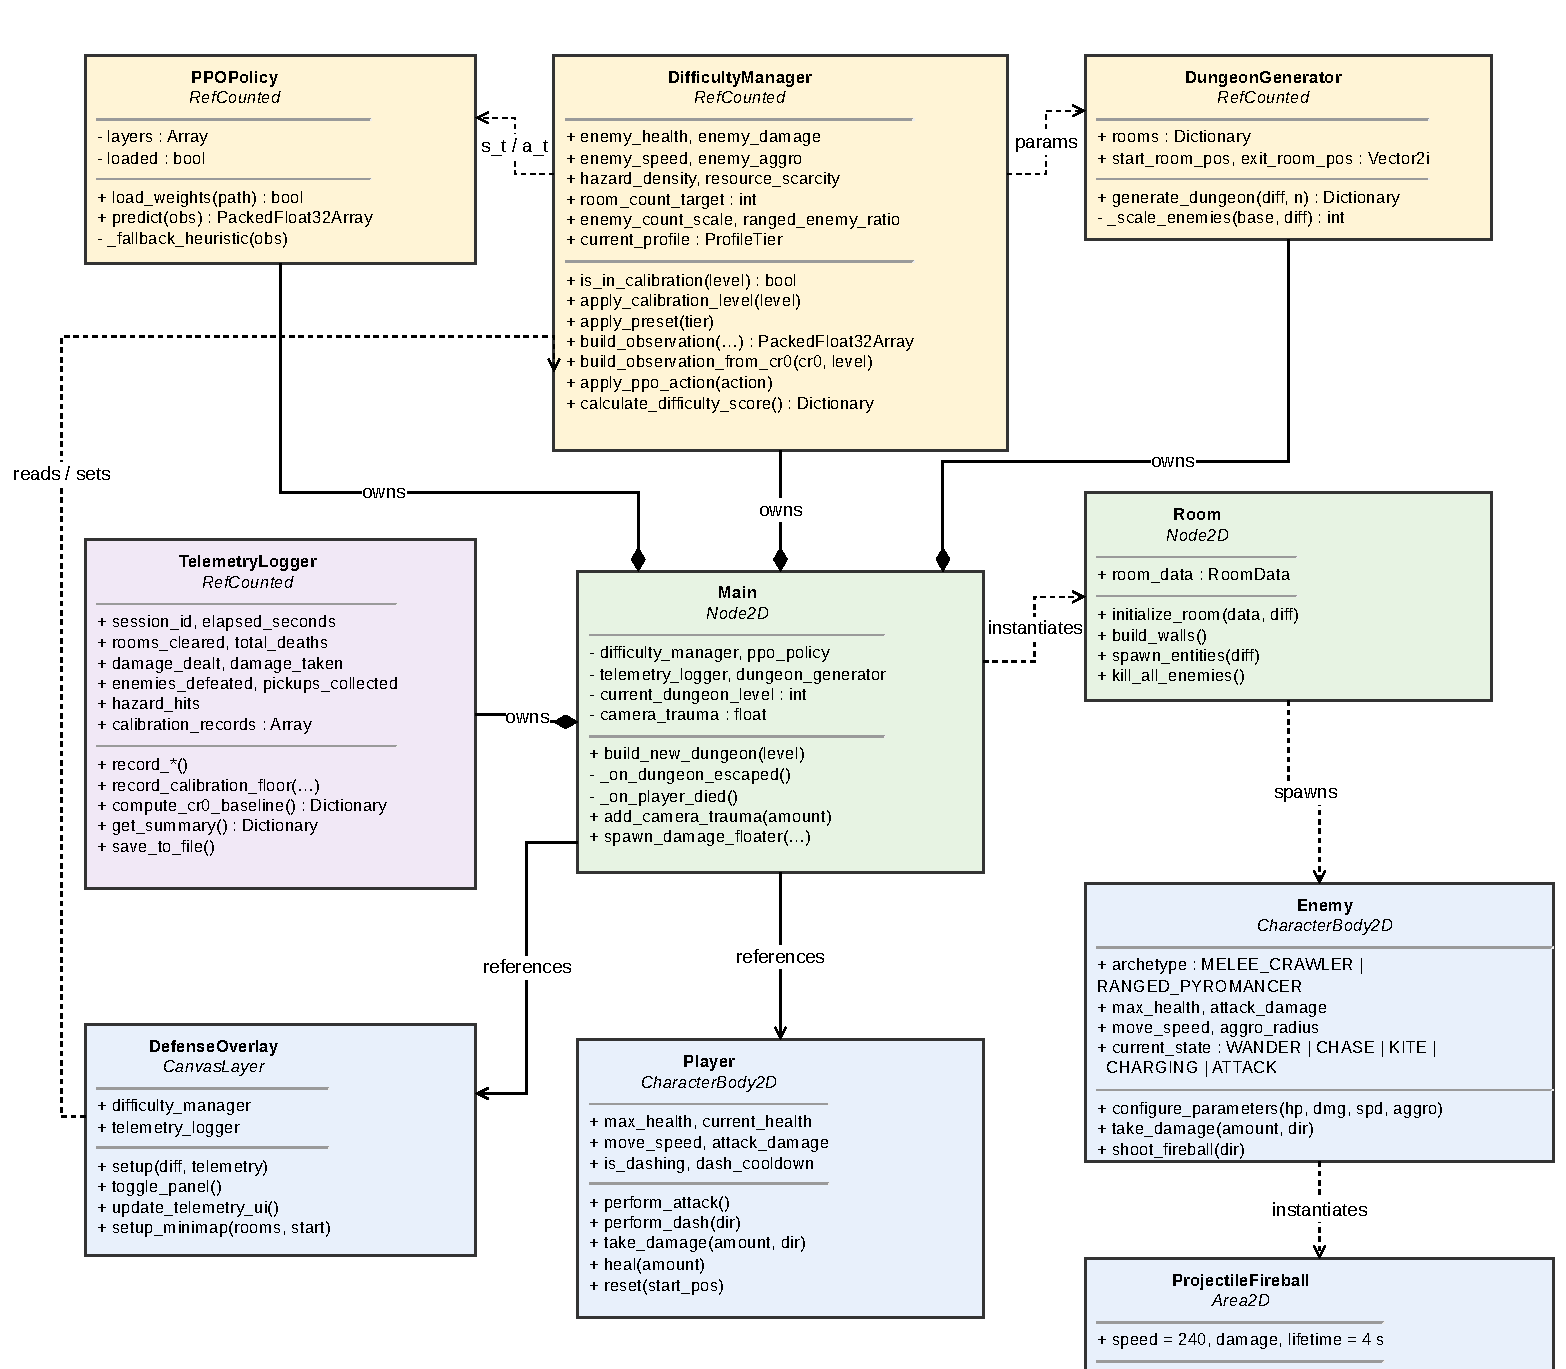
\includegraphics[width=0.98\textwidth]{ThesisFigs/fig_class_diagram}
\caption{UML Class Diagram of the Core Architecture (derived from the GDScript sources)}
\label{fig:class_diagram}
\end{figure}

\section{Data Design and Telemetry Schema}
\texttt{TelemetryLogger.gd} accumulates session metrics in memory and appends a snapshot (\texttt{get\_summary()}) to \texttt{user://session\_telemetry.json} after every room clear, every player death and every floor exit; the file keeps the most recent 50 snapshots. Table~\ref{tab:json_schema} lists the fields of one snapshot. The per-floor calibration records (floor, time, deaths, damage, rooms, difficulty score, seconds per room) are kept in memory and are used at the end of floor 5 to compute $CR_0$ and the seed observation $s_0$. Damage taken and dealt reach the logger through \texttt{Main.gd}'s \texttt{\_on\_player\_damaged} and \texttt{\_on\_enemy\_damaged} handlers (DEF-05).

\begin{table}[!htbp]
\centering
\caption[JSON Data Schema of a Telemetry Snapshot]{JSON Data Schema of a Telemetry Snapshot (\texttt{TelemetryLogger.get\_summary()})}
\label{tab:json_schema}
\small
\begin{tabular}{p{0.26\textwidth}p{0.14\textwidth}p{0.50\textwidth}}
\toprule
\textbf{Field Name} & \textbf{Data Type} & \textbf{Description \& Unit} \\
\midrule
\texttt{session\_id} & String & Session identifier of the form \texttt{sess\_<unix time>} \\
\texttt{timestamp} & Integer & Session start time (Unix seconds) \\
\texttt{elapsed\_seconds} & Float & Play time accumulated in the session (seconds) \\
\texttt{rooms\_cleared} & Integer & Rooms cleared so far \\
\texttt{total\_deaths} & Integer & Player deaths in the session \\
\texttt{damage\_dealt} & Float & Cumulative damage inflicted on enemies \\
\texttt{damage\_taken} & Float & Cumulative damage sustained by the player \\
\texttt{enemies\_defeated} & Integer & Enemies killed \\
\texttt{pickups\_collected} & Integer & Potions collected \\
\texttt{hazard\_hits} & Integer & Times the player was hit by a hazard \\
\texttt{exploration\_efficiency} & Float & Rooms cleared per minute \\
\bottomrule
\end{tabular}
\end{table}

\section{Process and Behavioral Design}

\subsection{Activity Diagram: Complete Game Session Lifecycle}
Figure~\ref{fig:activity_session} details the operational lifecycle of a gameplay session from menu initialization through cold-start calibration to closed-loop adaptive generation.

\begin{figure}[!htbp]
\centering
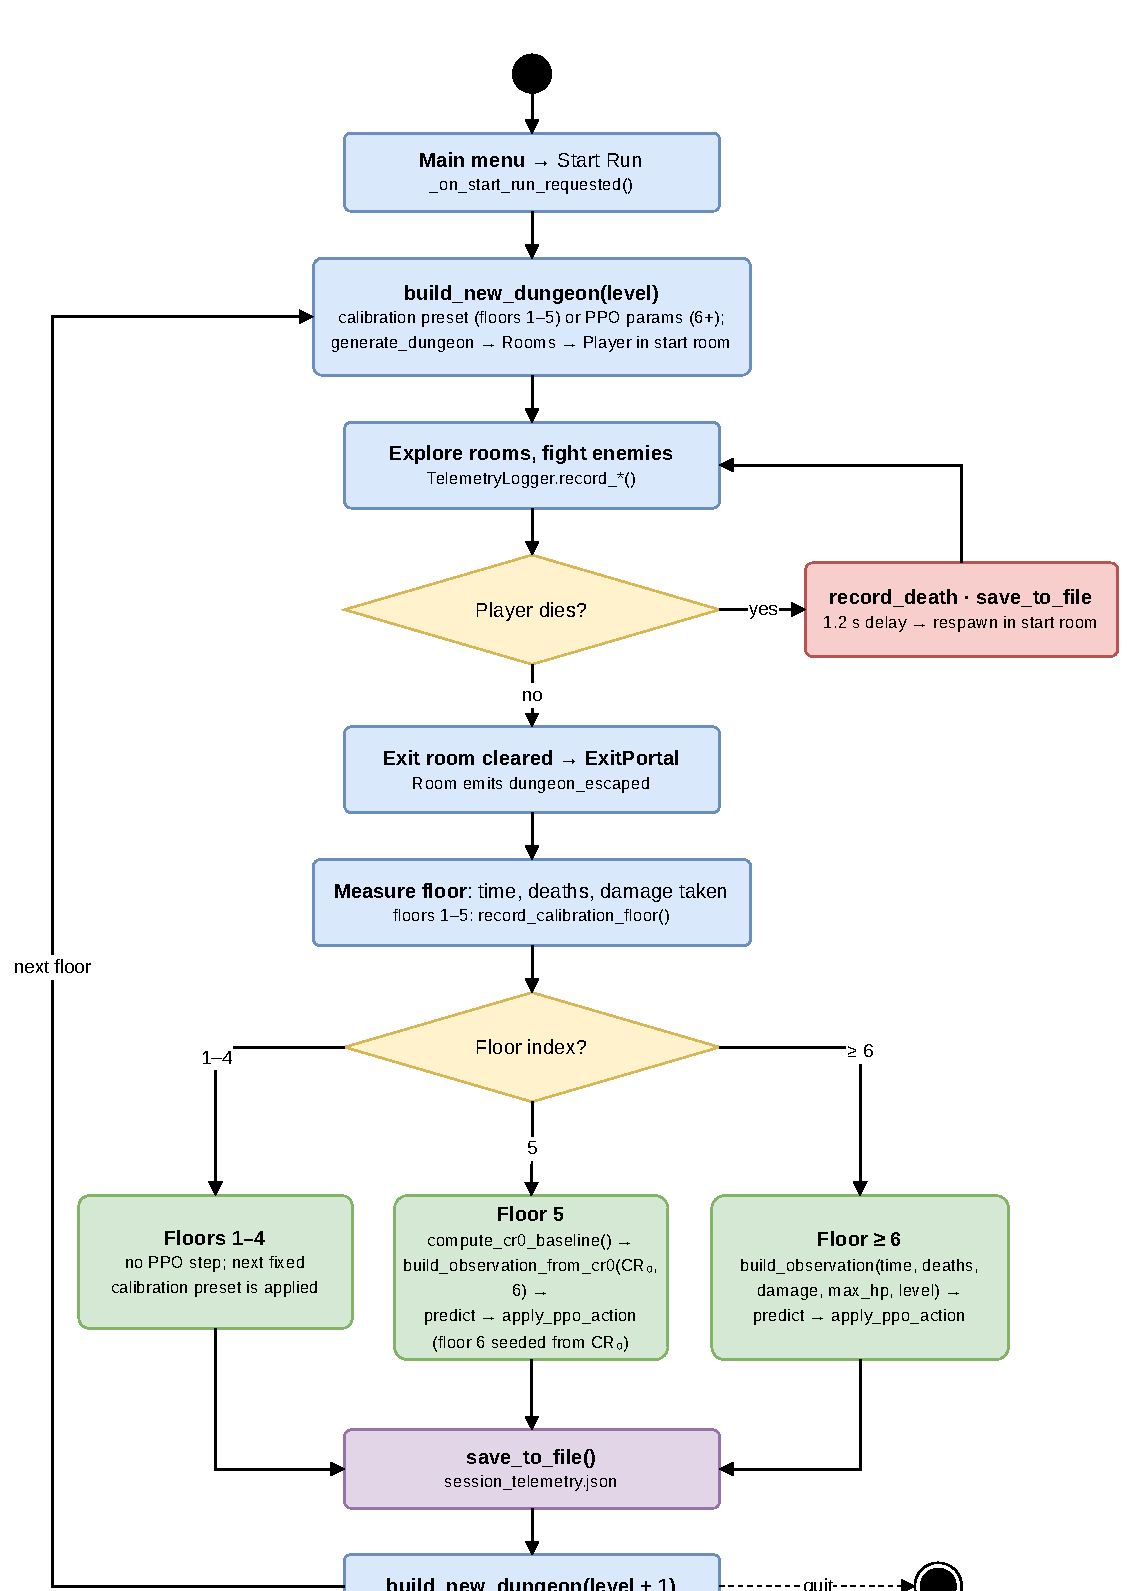
\includegraphics[width=0.65\textwidth, height=0.75\textheight, keepaspectratio]{ThesisFigs/fig_5_8_1_activity_diagram}
\caption{Activity Diagram Illustrating Complete Game Session Lifecycle}
\label{fig:activity_session}
\end{figure}

\subsection{Sequence Diagram: Inter-Floor Telemetry and Adaptation Cycle}
Figure~\ref{fig:seq_diagram} traces the message exchange when the player leaves a floor: calibration floors 1--4 only record telemetry, floor 5 computes $CR_0$ and seeds the first PPO action from the weighted calibration records ($s_0$, Equation~\ref{eq:s0_seed}), and floors 6 and above run one PPO step per floor.

\begin{figure}[!htbp]
\centering
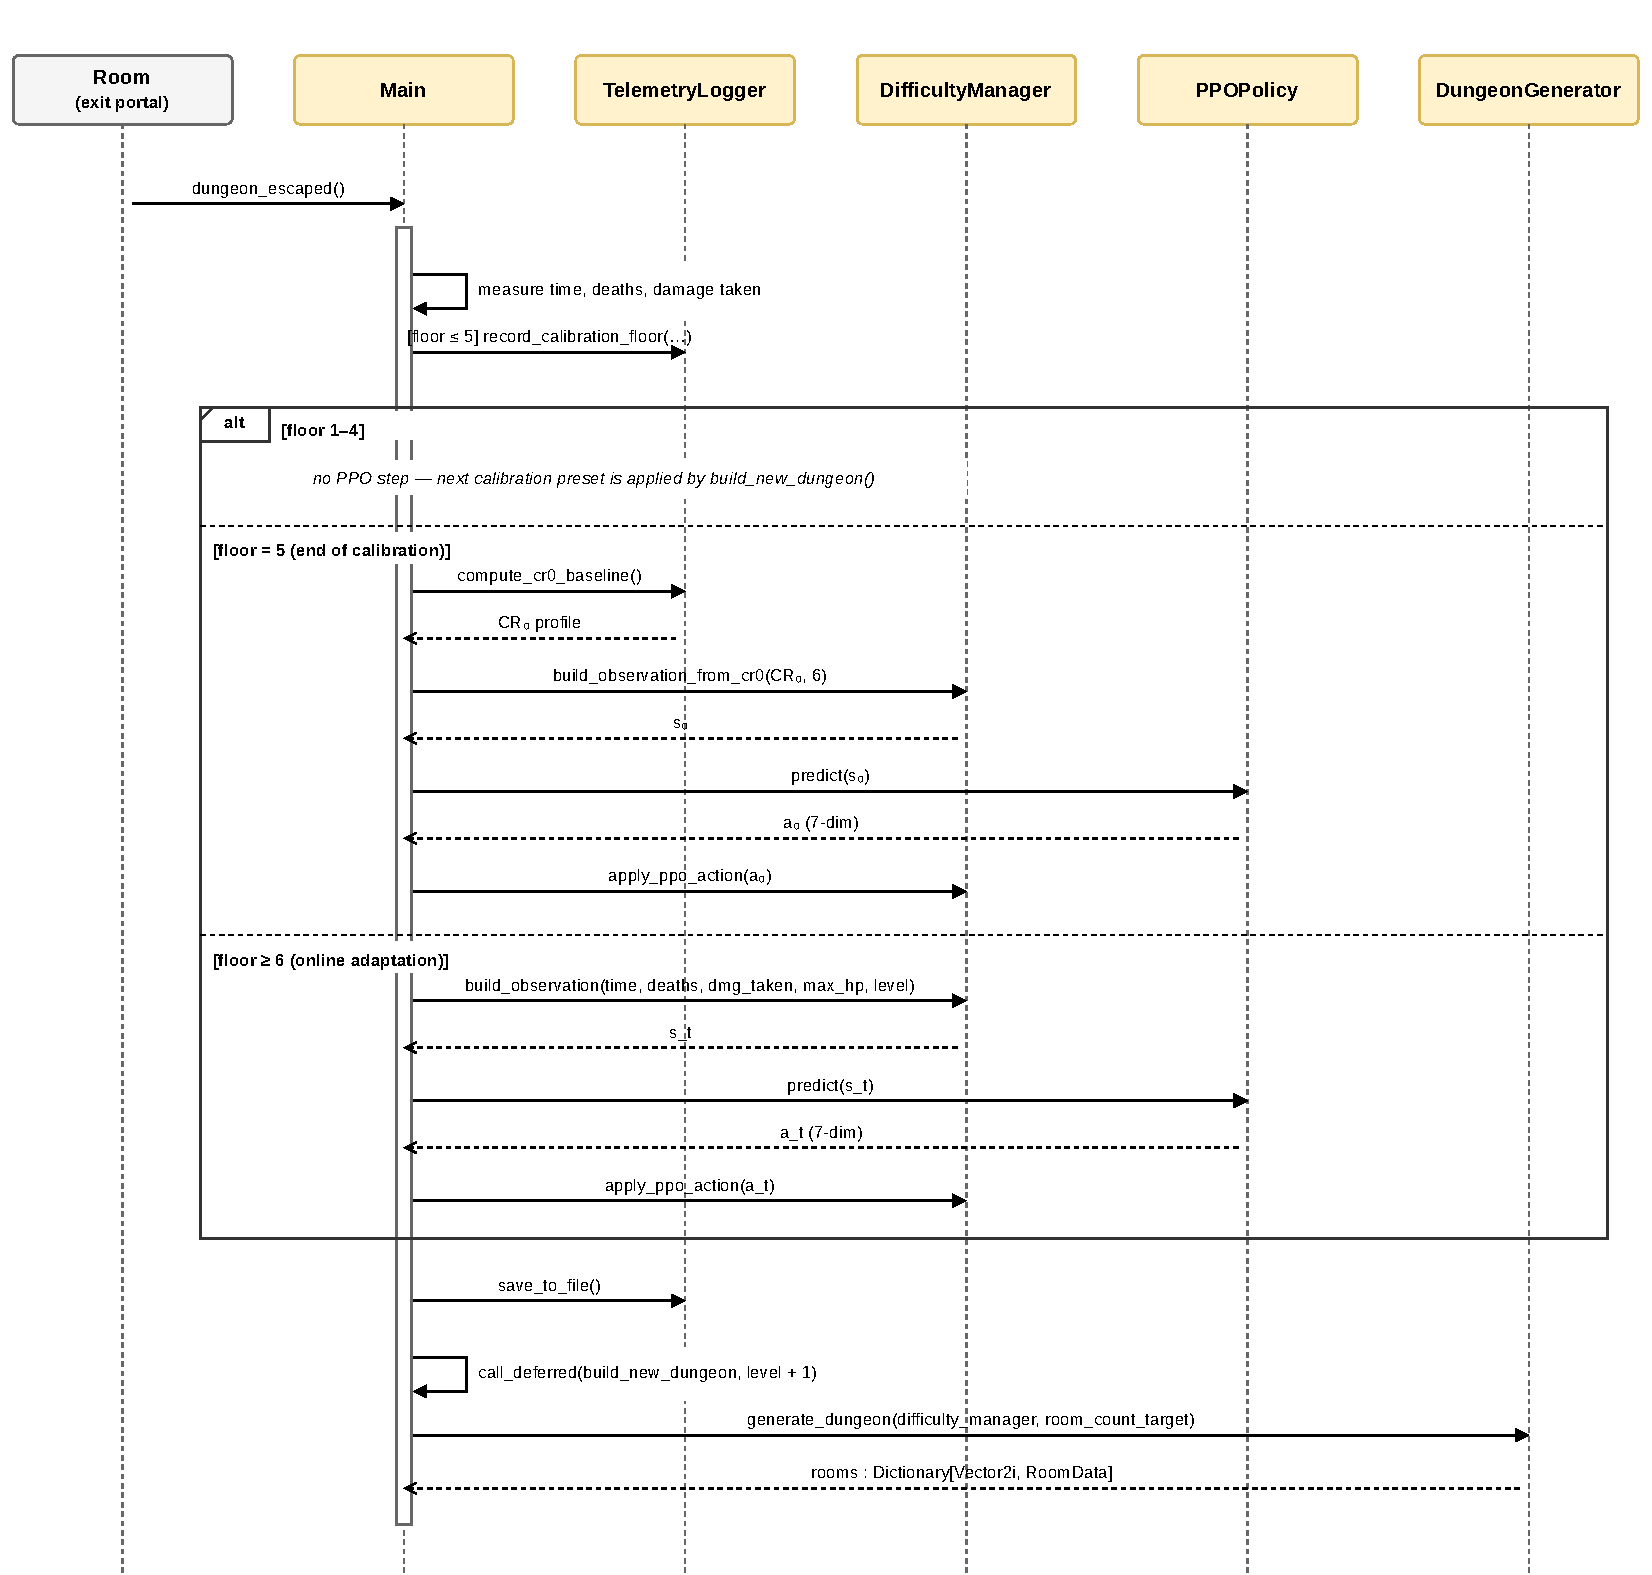
\includegraphics[width=0.98\textwidth]{ThesisFigs/fig_seq_inter_floor_adaptation}
\caption[UML Sequence Diagram of the Inter-Floor Adaptation Step]{UML Sequence Diagram of the Inter-Floor Adaptation Step (\texttt{Main.\_on\_dungeon\_escaped})}
\label{fig:seq_diagram}
\end{figure}

\subsection{State Machine Diagram: Enemy Combat AI}
Figure~\ref{fig:state_enemy} shows the finite state machines governing the two adversary archetypes in \texttt{Enemy.gd}. State changes are driven by the distance $d$ to the player rather than by timers, except for the Pyromancer's $0.5$\,s charge.

\begin{figure}[!htbp]
\centering
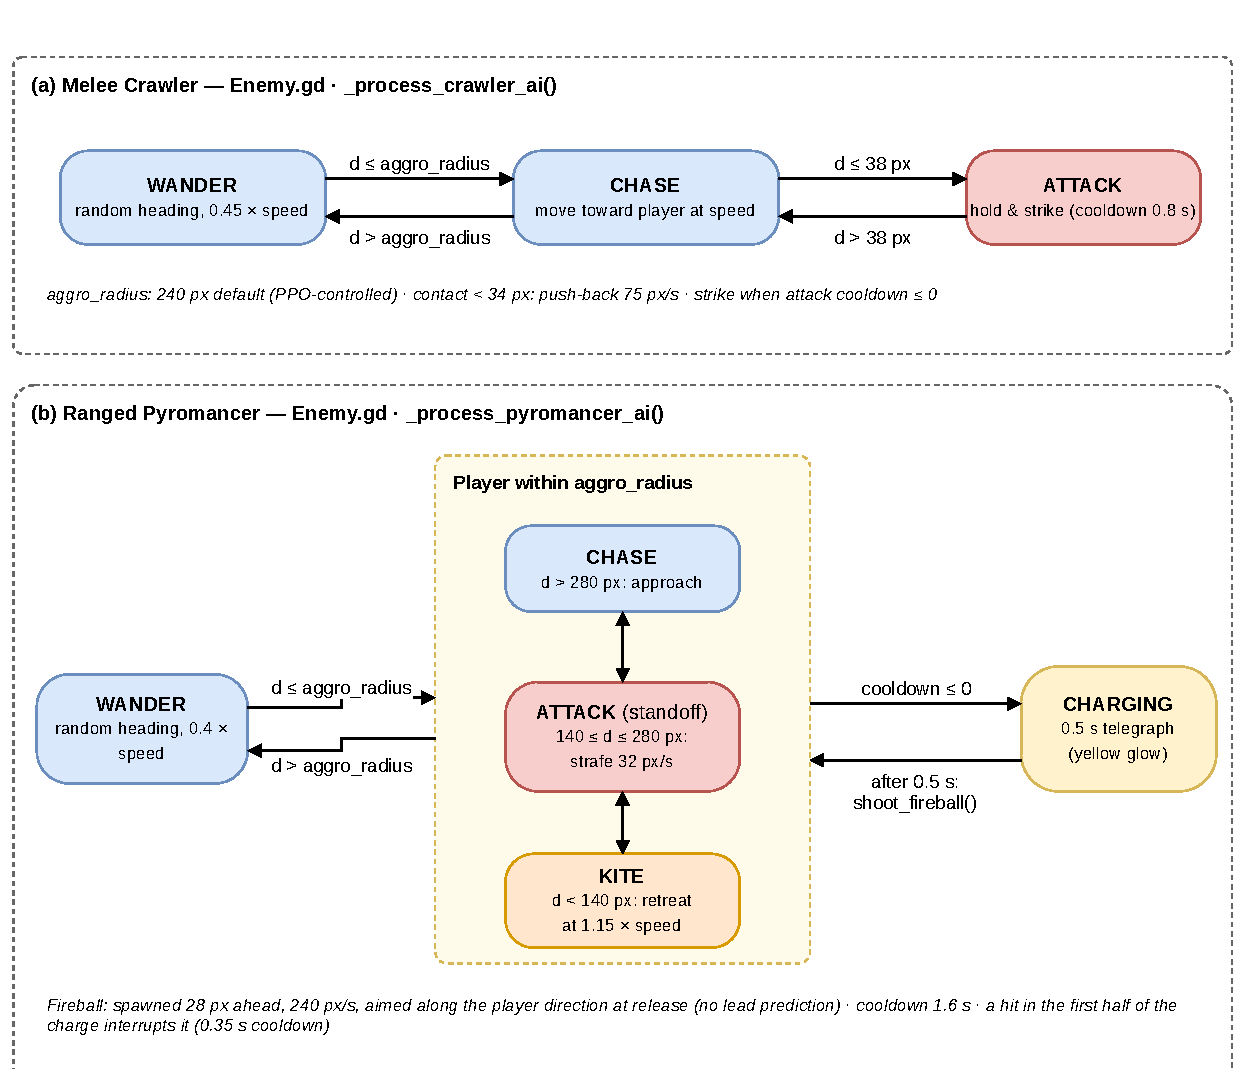
\includegraphics[width=0.85\textwidth]{ThesisFigs/fig_state_enemy_ai}
\caption[Finite State Machines of the Melee Crawler and Ranged Pyromancer]{Finite State Machines of the Melee Crawler and Ranged Pyromancer (\texttt{Enemy.gd})}
\label{fig:state_enemy}
\end{figure}
